\documentclass[border=4pt]{standalone}\usepackage[utf8]{inputenc}\usepackage[T1]{fontenc}\usepackage{mathptmx}
\usepackage{tikz}
\usetikzlibrary{arrows.meta,positioning,calc,fit,backgrounds}
\tikzset{>={Stealth[length=2.2mm]}, font=\small,
 blk/.style={draw, line width=0.8pt, fill=white, align=center, inner sep=3pt, text width=#1, minimum height=1.1cm},
 blk/.default=3.0cm,
 iut/.style={fill=black!14},
 ext/.style={draw, dashed, line width=0.5pt, align=center, inner sep=3pt, text width=#1, minimum height=1.0cm, fill=white},
 ext/.default=2.6cm,
 grp/.style={draw=black!55, dashed, line width=0.5pt, fill=black!4, inner sep=7pt},
 glab/.style={font=\small\itshape, text=black!75, anchor=north west, inner sep=2pt},
 lab/.style={font=\footnotesize, inner sep=1.5pt, fill=white},
 pw/.style={line width=2.2pt, -{Stealth[length=2.6mm]}},
 dg/.style={line width=0.6pt},
 an/.style={line width=0.8pt, dashed},
 rf/.style={double, double distance=1.2pt, line width=0.4pt},
 cd/.style={line width=0.6pt, dotted}}

\begin{document}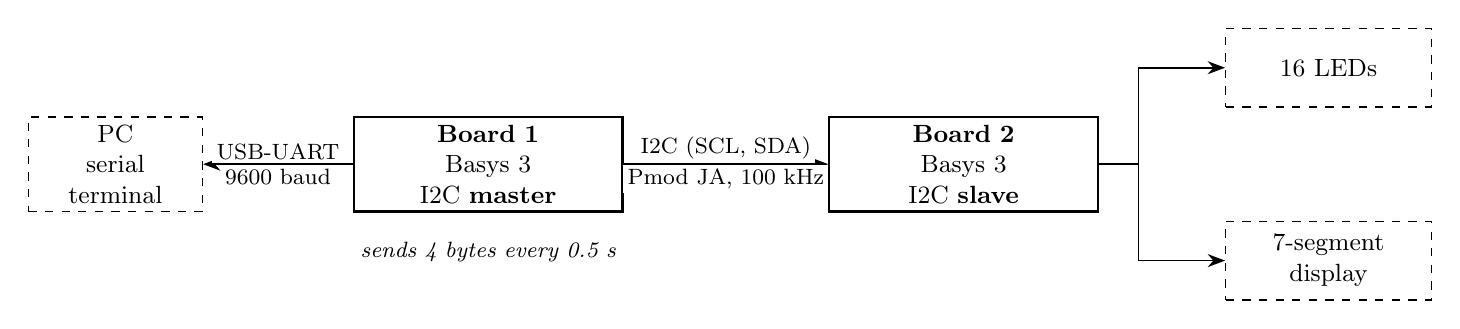
\begin{tikzpicture}
\node[ext=2.0cm] (pc) {PC\\serial terminal};
\node[blk=3.2cm, right=1.9cm of pc] (b1) {\textbf{Board 1}\\Basys 3\\I2C \textbf{master}};
\node[blk=3.2cm, right=2.6cm of b1] (b2) {\textbf{Board 2}\\Basys 3\\I2C \textbf{slave}};
\node[ext=2.4cm, above right=0.1cm and 1.6cm of b2] (led) {16 LEDs};
\node[ext=2.4cm, below right=0.1cm and 1.6cm of b2] (seg) {7-segment display};
\draw[dg,->] (b1) -- node[lab,above]{USB-UART} node[lab,below]{9600 baud} (pc);
\draw[dg,->] (b1) -- node[lab,above]{I2C (SCL, SDA)} node[lab,below]{Pmod JA, 100 kHz} (b2);
\draw[dg,->] (b2.east) -- ++(0.5,0) |- (led.west);
\draw[dg,->] (b2.east) -- ++(0.5,0) |- (seg.west);
\node[font=\footnotesize\itshape, below=0.25cm of b1, text width=3.6cm, align=center] {sends 4 bytes every 0.5 s};
\end{tikzpicture}\end{document}
